\documentclass[14pt]{extarticle}
\renewcommand{\theequation}{\Alph{equation}}
% \documentclass[14pt]{article}

% \usepackage[style=authoryear,maxbibnames=9,maxcitenames=2,uniquelist=false,backend=biber,doi=false,url=false]{biblatex}
% \addbibresource{$BIB} % bibtex location
% \renewcommand*{\nameyeardelim}{\addcomma\space} % have comma in parencite
\usepackage{natbib}

\usepackage{xcolor}
\usepackage{amsmath}
\newcommand{\tuple}[1]{ \langle #1 \rangle }
%\usepackage{automata}
\usepackage{times}
\usepackage{ltablex}
\usepackage{tasks}

%%%%%% Template
\usepackage{hyperref}
\hypersetup{colorlinks=true,allcolors=blue}

\usepackage{vmargin}
\setpapersize{USletter}
\setmarginsrb{1.0in}{1.0in}{1.0in}{0.6in}{0pt}{0pt}{0pt}{0.4in}

% HOW TO USE THE ABOVE:
%\setmarginsrb{leftmargin}{topmargin}{rightmargin}{bottommargin}{headheight}{headsep}{footheight}{footskip}
%\raggedbottom
% paragraphs indent & skip:
\parindent  0.3cm
\parskip    -0.01cm

\usepackage{tikz}
\usetikzlibrary{backgrounds}
\usetikzlibrary{decorations.pathreplacing, intersections, positioning}


% hyphenation:
% \hyphenpenalty=10000 % no hyphen
% \exhyphenpenalty=10000 % no hyphen
\sloppy

% notes-style paragraph spacing and indentation:
\usepackage{parskip}
\setlength{\parindent}{0cm}

% let derivations break across pages
\allowdisplaybreaks

\newcommand{\orange}[1]{\textcolor{orange}{#1}}
\newcommand{\blue}[1]{\textcolor{blue}{#1}}
\newcommand{\red}[1]{\textcolor{red}{#1}}
\newcommand{\freq}[1]{{\bf \sf F}(#1)}
\newcommand{\datafreq}[2]{{{\bf \sf F}_{#1}(#2)}}

\def\qqquad{\quad\qquad}
\def\qqqquad{\qquad\qquad}

%%%%%%%%%%%%%%%%%%%%%%%%%%%%%%%%%%%%%%%%%%%%%%%%%%%%%%%%%%%%%%%%%%%%%%%%%%%%%%%%
%%%%%%%%%%%%%%%%%%%%%%%%%%%%%%%%%%%%%%%%%%%%%%%%%%%%%%%%%%%%%%%%%%%%%%%%%%%%%%%%

% fill-in-blank question style, found in https://tex.stackexchange.com/a/505089

\usepackage{ifthen}
\usepackage{tocloft}
\usepackage{exercise}
% \usepackage{xcolor}

% Set the Show Answers Boolean
\newboolean{showAns}
\setboolean{showAns}{false}
\newcommand{\showAns}{\setboolean{showAns}{true}}

% The length of the Answer line
\newlength{\answerlength}
\newcommand{\anslen}[1]{\settowidth{\answerlength}{#1}}

% ans command that indicates space for an answer or shows the answer in red
\newcommand{\ans}[1]{\settowidth{\answerlength}{\hspace{2ex}#1\hspace{2ex}}%
    \ifthenelse{\boolean{showAns}}%
        {\textcolor{red}{\underline{\hspace{2ex}#1\hspace{2ex}}}}%
        {\underline{\hspace{\answerlength}}}}%

% Formatting how multiple choices Questions are formated.
\settasks{label=(\Alph*), label-width=30pt}


% Some commands for the Exercise Question package
\renewcommand{\QuestionNB}{\Large\protect\textcircled{\small\bfseries\arabic{Question}}\ }
\renewcommand{\ExerciseHeader}{} %no header
\renewcommand{\QuestionBefore}{3ex} %Space above each Q
\setlength{\QuestionIndent}{8pt} % Indent after Q number


% To create the list of answers with tocloft...
\newcommand{\listanswername}{Answers}
\newlistof[Question]{answer}{Answers}{\listanswername}

% Creates a TOC for Answers
\newcounter{prevQ}
\newcommand{\answer}[1]{\refstepcounter{answer}%
\ans{#1}%
\ifnum\theQuestion=\theprevQ%
        \addcontentsline{Answers}{answer}{\protect\numberline{}#1}% don't include the Q number
        \else%
        \addcontentsline{Answers}{answer}{\protect\numberline{\theQuestion}#1}%
        \setcounter{prevQ}{\value{Question}}%
        \fi%
        }%


%tocloft formatting listofanswers
\renewcommand{\cftAnswerstitlefont}{\bfseries\large}
\renewcommand{\cftanswerdotsep}{\cftnodots}
\cftpagenumbersoff{answer}
\addtolength{\cftanswernumwidth}{10pt}


%%%%%%%%%%%%%%%%%%%%%%%%%%%%%%%%%%%%%%%%%%%%%%%%%%%%%%%%%%%%%%%%%%%%%%%%%%%%%%%%
%%%%%%%%%%%%%%%%%%%%%%%%%%%%%%%%%%%%%%%%%%%%%%%%%%%%%%%%%%%%%%%%%%%%%%%%%%%%%%%%
\begin{document}

% \setcounter{section}{}
\centerline{\huge\bf ECON 4002.01 Final Exam}
\smallskip
\centerline{\LARGE Hui-Jun Chen}

\medskip

% \showAns
% \listofanswer

\begin{Exercise}

\section*{Question 1}
\label{sec:Question_1}
\addcontentsline{toc}{section}{Question 1}



Consider the two-period dynamic general equilibrium model with a representative consumer, representative firm and government.
The consumer values consumption and leisure in each period, $C$ and $l$, and provides labour, $N_{S}$, in return for a real wage, $w$. The consumer pays lump-sum taxes $ T $ each period and receives all profits from the firm, $\pi$.%

The representative firm uses labour and capital, $N_{D}$ and $K$, to produce output.
In the first period, it also chooses investment, $I$.
This determines its capital stock for production in the second period, $K^{\prime}$, through the capital accumulation equation $K^{\prime}=\left(  1-\delta\right)  K+I$.%

The consumer's preferences are
%
\begin{equation*}
    U(C, C', N, N') = u(C) - v(N_{S}) + u(C') - v(N_{S})
,\end{equation*}
%
and the firm's technology is
%
\begin{equation*}
    Y = z F(K, N) = z K^{\alpha} N^{1-\alpha}, \text{ where } \alpha \in (0, 1)
.\end{equation*}
%
Lastly, recall that the government must balance its budget across the two periods, $G+\frac{G^{\prime}}{1+r}=T+\frac{T^{\prime} }{1+r}$, where $G$ is government spending and $T$ are taxes.



\Question \label{MRS} Assume assumption N1 holds, i.e., substitution effect dominates income effect from a change in real wage, then given interest rate $ r $, consumer will choose the quantity of labor supply $ N_{S} $ by \answer{A}
\begin{tasks}(2)
    \task $ MRS_{l, C} = w $
    \task $ MRS_{C, C'} = r $
    \task $ MRS_{l, C} = r $
    \task $ MRS_{C, C'} = w $
\end{tasks}

\Question where the $ MRS $ in question \ref{MRS} is \answer{C}
\begin{tasks}(2)
    \task $ MRS_{l, C} = \frac{u'(C)}{u'(C')} $
    \task $ MRS_{C, C'} = \frac{u'(C)}{u'(C')}$
    \task $ MRS_{l, C} = \frac{v'(N_{S})}{u'(C)} $
    \task $ MRS_{C, C'} = \frac{v'(N_{S})}{u'(C)} $
\end{tasks}

\Question Following assumption N1, the slope of the labor supply is \answer{D} in wage and thus the labor supply curve has \answer{D} slope
\begin{tasks}(2)
    \task decreasing; positive
    \task increasing; negative
    \task decreasing; negative
    \task increasing; positive
\end{tasks}

\Question Following assumption N2, how does the labor supply curve response to a rise in real interest rate $ r $? \answer{B}
\begin{tasks}(2)
    \task shift to the left
    \task shift to the right
    \task not affected
    \task ambiguous
\end{tasks}

\Question In the firm's labor demand, what is the equation that can determine the labor demand curve? \answer{A}
\begin{tasks}(2)
    \task $ MPN = w $
    \task $ MPK = r $
    \task $ MPN = r $
    \task $ MPK = w $
\end{tasks}


\Question How does a fall in total factor productivity $ z $ affect the equilibrium in labor market? \answer{B}
\begin{tasks}(1)
    \task labor supply will shift to the left; labor demand will shift to the right
    \task labor supply will shift to the right; labor demand will shift to the left
    \task labor supply will shift to the right; labor demand not shift
    \task labor supply will not shift; labor demand will shift to the left
\end{tasks}

\Question For the goods demand, what is the optimal investment schedule? \answer{D}
\begin{tasks}(2)
    \task $ MPN' - \delta = w $
    \task $ MPN' - \delta = r $
    \task $ MPK' - w = r $
    \task $ MPK' - \delta = r $
\end{tasks}

\Question how does a rise in the real interest rate $ r $ changes the investment? \answer{C}
\begin{tasks}(2)
    \task $ I^{d} \uparrow  $
    \task $ I^{d} $ unchanged
    \task $ I^{d} \downarrow  $
    \task $ I^{d} $ movement is ambiguous
\end{tasks}

% A: z', B: z, C: K, D: G
\Question \label{z'} Consider a rise in future total factor productivity $ z' $. Which of the following figure correctly represents the movement of labor and goods market? \answer{A}
\begin{tasks}(1)
    \task

        \begin{minipage}{0.5\textwidth}
            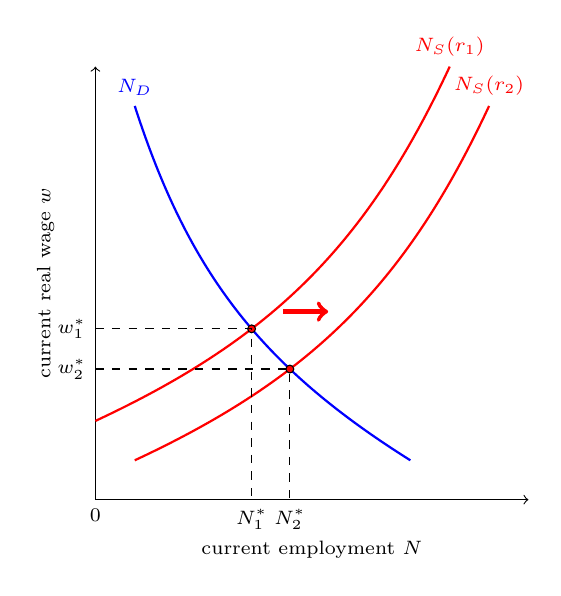
\begin{tikzpicture}[domain=0:5]
                \tikzstyle{every node}=[font=\scriptsize]
                \pgfmathsetmacro{\x}{5};
                \pgfmathsetmacro{\y}{5};
                % \draw[very thin,color=gray, step=0.1] (0,0) grid (\x, \y); % gray grid
                \draw[->] (0,0) node[below]{ $ 0 $  } -- node[below, yshift = -0.4cm]{current employment $ N $} (\x + 0.5,0) ;   % label x axis
                \draw[->] (0,0) -- node[above, rotate=90, yshift = 0.4cm]{current real wage $w$} (0,\y + 0.5) ;   % label y axis
                \draw[thick, red, xshift = -0.5cm, yshift = 0.5cm, name path = aaa]
                    (\x, \y)
                    node[above]{$N_{S}( r_{1} )$}
                    to[bend left=20]
                    node[pos=0.6] (AA) {}
                    (0.5, 0.5);
                \draw[thick, red, name path = aa]
                    (\x, \y)
                    node[above]{$N_{S}( r_{2} )$}
                    to[bend left=20]
                    (0.5, 0.5);
                \draw[thick, blue, name path = bb]
                    (0.5, \y)
                    node[above]{$N_{D}$}
                    to[bend right=20]
                    (4, 0.5);
                \path[name intersections={of=aa and bb, by=b}];
                \path[name intersections={of=aaa and bb, by=bb}];
                \node[draw,fill=red,circle,inner sep=1pt] at (b) {};
                \node[draw,fill=red,circle,inner sep=1pt] at (bb) {};
                \draw[->, ultra thick, red] (AA) -- ++(0.7, 0);
                \path (bb); \pgfgetlastxy{\xcoord}{\ycoord};
                \coordinate (bb_x) at (\xcoord, 0);
                \coordinate (bb_y) at (0, \ycoord);
                \draw[dashed] (bb_y) node[left]{$w_{1}^{*}$}  -- (bb) -- (bb_x) node[below]{$N_{1}^{*}$};
                \path (b); \pgfgetlastxy{\xcoord}{\ycoord};
                \coordinate (b_x) at (\xcoord, 0);
                \coordinate (b_y) at (0, \ycoord);
                \draw[dashed] (b_y) node[left]{$w_{2}^{*}$}  -- (b) -- (b_x) node[below]{$N_{2}^{*}$};

            \end{tikzpicture}
        \end{minipage}
        \begin{minipage}{0.5\textwidth}

            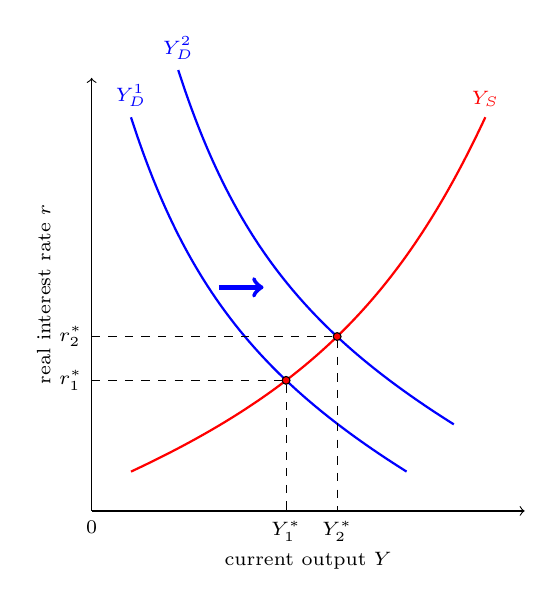
\begin{tikzpicture}[domain=0:5]
                \tikzstyle{every node}=[font=\scriptsize]
                \pgfmathsetmacro{\x}{5};
                \pgfmathsetmacro{\y}{5};
                % \draw[very thin,color=gray, step=0.1] (0,0) grid (\x, \y); % gray grid
                \draw[->] (0,0) node[below]{ $ 0 $  } -- node[below, yshift = -0.4cm]{current output $ Y $} (\x + 0.5,0) ;   % label x axis
                \draw[->] (0,0) -- node[above, rotate=90, yshift = 0.4cm]{real interest rate $r$} (0,\y + 0.5) ;   % label y axis
                \draw[thick, red, name path = aa]
                    (\x, \y)
                    node[above]{$Y_{S}$}
                    to[bend left=20]
                    (0.5, 0.5);
                \draw[thick, blue, name path = bb]
                    (0.5, \y)
                    node[above]{$Y_{D}^{1}$}
                    to[bend right=20]
                    node[pos = 0.4] (BB) {}
                    (4, 0.5);
                \draw[thick, blue, xshift = 0.6cm, yshift = 0.6cm, name path = bbb]
                    (0.5, \y)
                    node[above]{$Y_{D}^{2}$}
                    to[bend right=20]
                    (4, 0.5);
                \path[name intersections={of=aa and bb, by=a}];
                \path[name intersections={of=aa and bbb, by=bbb}];
                \node[draw,fill=red,circle,inner sep=1pt] at (a) {};
                \node[draw,fill=red,circle,inner sep=1pt] at (bbb) {};
                \draw[->, ultra thick, blue] (BB) -- ++(0.7, 0);
                \path (a); \pgfgetlastxy{\xcoord}{\ycoord};
                \coordinate (a_x) at (\xcoord, 0);
                \coordinate (a_y) at (0, \ycoord);
                \draw[dashed] (a_y) node[left]{$r_{1}^{*}$}  -- (a) -- (a_x) node[below]{$Y_{1}^{*}$};
                \path (bbb); \pgfgetlastxy{\xcoord}{\ycoord};
                \coordinate (bbb_x) at (\xcoord, 0);
                \coordinate (bbb_y) at (0, \ycoord);
                \draw[dashed] (bbb_y) node[left]{$r_{2}^{*}$}  -- (bbb) -- (bbb_x) node[below]{$Y_{2}^{*}$};

            \end{tikzpicture}
        \end{minipage}

    \task

        \begin{minipage}{0.5\textwidth}
            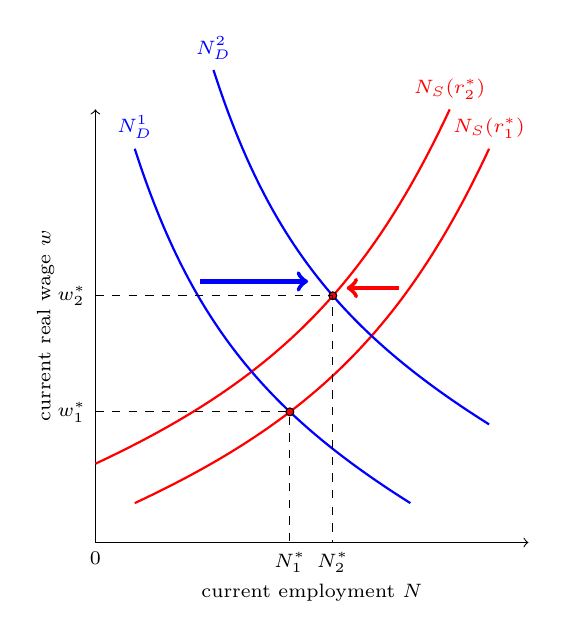
\begin{tikzpicture}[domain=0:5]
                \tikzstyle{every node}=[font=\scriptsize]
                \pgfmathsetmacro{\x}{5};
                \pgfmathsetmacro{\y}{5};
                % \draw[very thin,color=gray, step=0.1] (0,0) grid (\x, \y); % gray grid
                \draw[->] (0,0) node[below]{ $ 0 $  } -- node[below, yshift = -0.4cm]{current employment $ N $} (\x + 0.5,0) ;   % label x axis
                \draw[->] (0,0) -- node[above, rotate=90, yshift = 0.4cm]{current real wage $w$} (0,\y + 0.5) ;   % label y axis
                \draw[thick, red, name path = aa]
                    (\x, \y)
                    node[above]{$N_{S}( r_{1}^{*} )$}
                    to[bend left=20]
                    node[pos=0.3] (AA) {}
                    (0.5, 0.5);
                \draw[thick, red, xshift = -0.5cm, yshift = 0.5cm, name path = dd]
                    (\x, \y)
                    node[above]{$N_{S}( r_{2}^{*} )$}
                    to[bend left=20]
                    (0.5, 0.5);
                \draw[thick, blue, name path = bb]
                    (0.5, \y)
                    node[above]{$N_{D}^{1}$}
                    to[bend right=20]
                    node[pos=0.3] (BB) {}
                    (4, 0.5);
                \draw[thick, blue, xshift = 1cm, yshift = 1cm, name path = cc]
                    (0.5, \y)
                    node[above]{$N_{D}^{2}$}
                    to[bend right=20]
                    (4, 0.5);
                \path[name intersections={of=aa and bb, by=b}];
                \path[name intersections={of=dd and cc, by=c}];
                \node[draw,fill=red,circle,inner sep=1pt] at (b) {};
                \node[draw,fill=red,circle,inner sep=1pt] at (c) {};
                \draw[->, ultra thick, blue] (BB) -- ++(1.5, 0);
                \draw[->, ultra thick, red] (AA) -- ++(-0.8, 0);
                \path (b); \pgfgetlastxy{\xcoord}{\ycoord};
                \coordinate (b_x) at (\xcoord, 0);
                \coordinate (b_y) at (0, \ycoord);
                \path (c); \pgfgetlastxy{\xcoord}{\ycoord};
                \coordinate (c_x) at (\xcoord, 0);
                \coordinate (c_y) at (0, \ycoord);
                \draw[dashed] (b_y) node[left]{$w_{1}^{*}$}  -- (b) -- (b_x) node[below]{$N_{1}^{*}$};
                \draw[dashed] (c_y) node[left]{$w_{2}^{*}$}  -- (c) -- (c_x) node[below]{$N_{2}^{*}$};

            \end{tikzpicture}
        \end{minipage}
        \begin{minipage}{0.5\textwidth}

            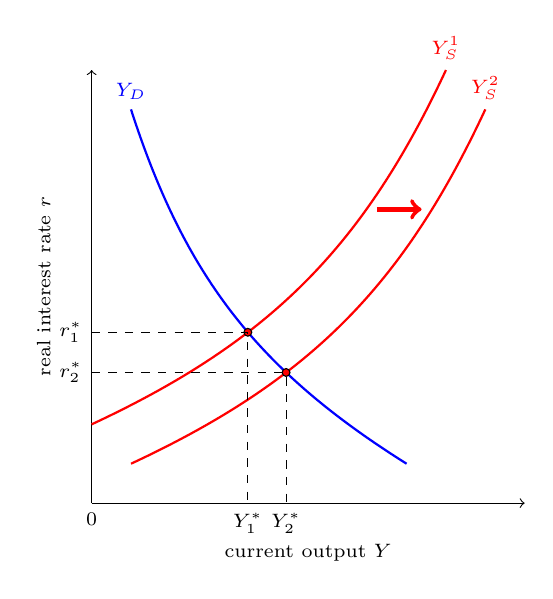
\begin{tikzpicture}[domain=0:5]
                \tikzstyle{every node}=[font=\scriptsize]
                \pgfmathsetmacro{\x}{5};
                \pgfmathsetmacro{\y}{5};
                % \draw[very thin,color=gray, step=0.1] (0,0) grid (\x, \y); % gray grid
                \draw[->] (0,0) node[below] {$ 0 $} -- node[below, yshift = -0.4cm]{current output $ Y $} (\x + 0.5,0) ;   % label x axis
                \draw[->] (0,0) -- node[above, rotate=90, yshift = 0.4cm]{real interest rate $r$} (0,\y + 0.5) ;   % label y axis
                \draw[thick, red, name path = aa]
                    (\x, \y)
                    node[above]{$Y_{S}^{2}$}
                    to[bend left=20]
                    (0.5, 0.5);
                \draw[thick, red, xshift = -0.5cm, yshift = 0.5cm, name path = cc]
                    (\x, \y)
                    node[above]{$Y_{S}^{1}$}
                    to[bend left=20]
                    node[pos=0.3] (AA) {}
                    (0.5, 0.5);
                \draw[thick, blue, name path = bb]
                    (0.5, \y)
                    node[above]{$Y_{D}$}
                    to[bend right=20]
                    (4, 0.5);
                \path[name intersections={of=aa and bb, by=a}];
                \path[name intersections={of=bb and cc, by=c}];
                \node[draw,fill=red,circle,inner sep=1pt] at (a) {};
                \node[draw,fill=red,circle,inner sep=1pt] at (c) {};
                \draw[->, ultra thick, red] (AA) -- ++(0.7, 0);
                \path (a); \pgfgetlastxy{\xcoord}{\ycoord};
                \coordinate (a_x) at (\xcoord, 0);
                \coordinate (a_y) at (0, \ycoord);
                \path (c); \pgfgetlastxy{\xcoord}{\ycoord};
                \coordinate (c_x) at (\xcoord, 0);
                \coordinate (c_y) at (0, \ycoord);
                \draw[dashed] (a_y) node[left]{$r_{2}^{*}$}  -- (a) -- (a_x) node[below]{$Y_{2}^{*}$};
                \draw[dashed] (c_y) node[left]{$r_{1}^{*}$}  -- (c) -- (c_x) node[below]{$Y_{1}^{*}$};
            \end{tikzpicture}
        \end{minipage}

    \task

        \begin{minipage}{0.5\textwidth}
            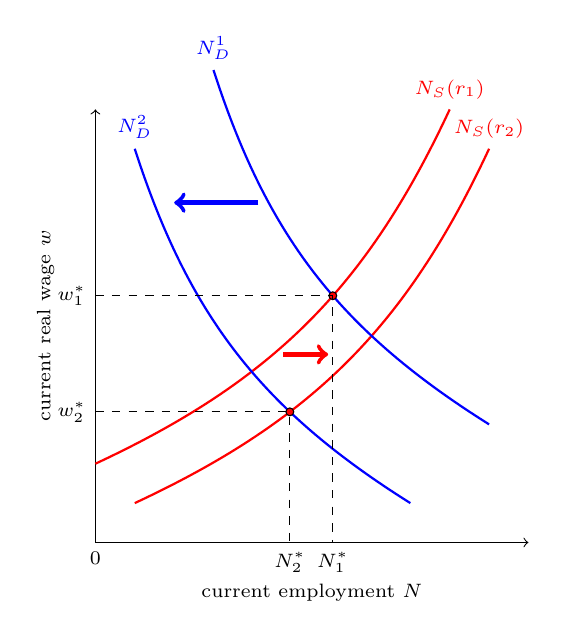
\begin{tikzpicture}[domain=0:5]
                \tikzstyle{every node}=[font=\scriptsize]
                \pgfmathsetmacro{\x}{5};
                \pgfmathsetmacro{\y}{5};
                % \draw[very thin,color=gray, step=0.1] (0,0) grid (\x, \y); % gray grid
                \draw[->] (0,0) node[below]{ $ 0 $  } -- node[below, yshift = -0.4cm]{current employment $ N $} (\x + 0.5,0) ;   % label x axis
                \draw[->] (0,0) -- node[above, rotate=90, yshift = 0.4cm]{current real wage $w$} (0,\y + 0.5) ;   % label y axis
                \draw[thick, red, xshift = -0.5cm, yshift = 0.5cm, name path = aaa]
                    (\x, \y)
                    node[above]{$N_{S}( r_{1} )$}
                    to[bend left=20]
                    node[pos=0.6] (AA) {}
                    (0.5, 0.5);
                \draw[thick, red, name path = aa]
                    (\x, \y)
                    node[above]{$N_{S}( r_{2} )$}
                    to[bend left=20]
                    (0.5, 0.5);
                \draw[thick, blue, xshift = 1cm, yshift = 1cm, name path = bbb]
                    (0.5, \y)
                    node[above]{$N_{D}^{1}$}
                    to[bend right=20]
                    node[pos = 0.3] (BB) {}
                    (4, 0.5);
                \draw[thick, blue, name path = bb]
                    (0.5, \y)
                    node[above]{$N_{D}^{2}$}
                    to[bend right=20]
                    (4, 0.5);
                \path[name intersections={of=aa and bb, by=b}];
                \path[name intersections={of=aaa and bbb, by=bb}];
                \node[draw,fill=red,circle,inner sep=1pt] at (b) {};
                \node[draw,fill=red,circle,inner sep=1pt] at (bb) {};
                \draw[->, ultra thick, red] (AA) -- ++(0.7, 0);
                \draw[->, ultra thick, blue] (BB) -- ++(-1.2, 0);
                \path (bb); \pgfgetlastxy{\xcoord}{\ycoord};
                \coordinate (bb_x) at (\xcoord, 0);
                \coordinate (bb_y) at (0, \ycoord);
                \draw[dashed] (bb_y) node[left]{$w_{1}^{*}$}  -- (bb) -- (bb_x) node[below]{$N_{1}^{*}$};
                \path (b); \pgfgetlastxy{\xcoord}{\ycoord};
                \coordinate (b_x) at (\xcoord, 0);
                \coordinate (b_y) at (0, \ycoord);
                \draw[dashed] (b_y) node[left]{$w_{2}^{*}$}  -- (b) -- (b_x) node[below]{$N_{2}^{*}$};

            \end{tikzpicture}
        \end{minipage}
        \begin{minipage}{0.5\textwidth}

            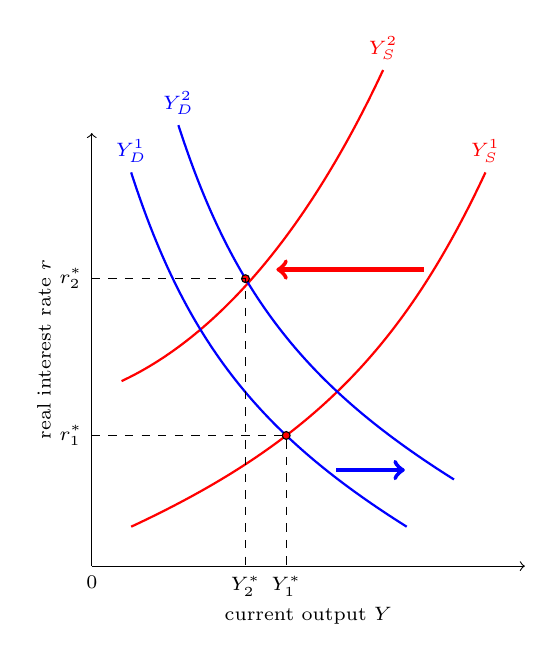
\begin{tikzpicture}[domain=0:5]
                \tikzstyle{every node}=[font=\scriptsize]
                \pgfmathsetmacro{\x}{5};
                \pgfmathsetmacro{\y}{5};
                % \draw[very thin,color=gray, step=0.1] (0,0) grid (\x, \y); % gray grid
                \draw[->] (0,0) node[below]{ $ 0 $  } -- node[below, yshift = -0.4cm]{current output $ Y $} (\x + 0.5,0) ;   % label x axis
                \draw[->] (0,0) -- node[above, rotate=90, yshift = 0.4cm]{real interest rate $r$} (0,\y + 0.5) ;   % label y axis
                \draw[thick, red, name path = aa]
                    (\x, \y)
                    node[above]{$Y_{S}^{1}$}
                    to[bend left=20]
                    node[pos = 0.2] (AA) {}
                    (0.5, 0.5);
                \draw[thick, red, xshift = -1.3cm, yshift = 1.3cm, name path = aaa, shorten >= 1.3cm]
                    (\x, \y)
                    node[above]{$Y_{S}^{2}$}
                    to[bend left=20]
                    (0.5, 0.5);
                \draw[thick, blue, name path = bb]
                    (0.5, \y)
                    node[above]{$Y_{D}^{1}$}
                    to[bend right=20]
                    node[pos = 0.8] (BB) {}
                    (4, 0.5);
                \draw[thick, blue, xshift = 0.6cm, yshift = 0.6cm, name path = bbb]
                    (0.5, \y)
                    node[above]{$Y_{D}^{2}$}
                    to[bend right=20]
                    (4, 0.5);
                \path[name intersections={of=aa and bb, by=a}];
                \path[name intersections={of=aaa and bbb, by=bbb}];
                \node[draw,fill=red,circle,inner sep=1pt] at (a) {};
                \node[draw,fill=red,circle,inner sep=1pt] at (bbb) {};
                \draw[->, ultra thick, blue] (BB) -- ++(1, 0);
                \draw[->, ultra thick, red] (AA) -- ++(-2, 0);
                \path (a); \pgfgetlastxy{\xcoord}{\ycoord};
                \coordinate (a_x) at (\xcoord, 0);
                \coordinate (a_y) at (0, \ycoord);
                \draw[dashed] (a_y) node[left]{$r_{1}^{*}$}  -- (a) -- (a_x) node[below]{$Y_{1}^{*}$};
                \path (bbb); \pgfgetlastxy{\xcoord}{\ycoord};
                \coordinate (bbb_x) at (\xcoord, 0);
                \coordinate (bbb_y) at (0, \ycoord);
                \draw[dashed] (bbb_y) node[left]{$r_{2}^{*}$}  -- (bbb) -- (bbb_x) node[below]{$Y_{2}^{*}$};

            \end{tikzpicture}
        \end{minipage}

    \task

        \begin{minipage}{0.5\textwidth}
            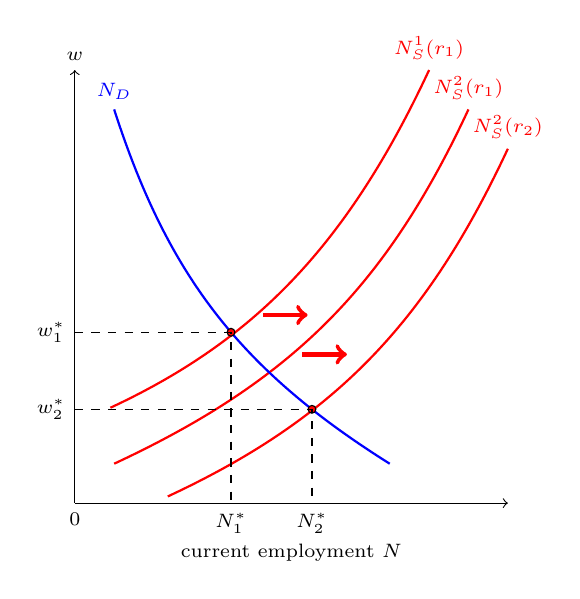
\begin{tikzpicture}[domain=0:5]
                \tikzstyle{every node}=[font=\scriptsize]
                \pgfmathsetmacro{\x}{5};
                \pgfmathsetmacro{\y}{5};
                % \draw[very thin,color=gray, step=0.1] (0,0) grid (\x, \y); % gray grid
                \draw[->] (0,0) node[below]{ $ 0 $  } -- node[below, yshift = -0.4cm]{current employment $ N $} (\x + 0.5,0) ;   % label x axis
                \draw[->] (0,0) -- (0,\y + 0.5) node[above]{$w$} ;   % label y axis
                \draw[thick, red, xshift = -0.5cm, yshift = 0.5cm, name path = aaa, shorten >= 0.5cm]
                    (\x, \y)
                    node[above]{$N_{S}^{1}( r_{1} )$}
                    to[bend left=20]
                    node[pos=0.6] (AA) {}
                    (0.5, 0.5);
                \draw[thick, red, name path = aa]
                    (\x, \y)
                    node[above]{$N_{S}^{2}( r_{1} )$}
                    to[bend left=20]
                    node[pos=0.6] (AAA) {}
                    (0.5, 0.5);
                \draw[thick, red, xshift = 0.5cm, yshift = -0.5cm, name path = aaaa, shorten >= 0.2cm]
                    (\x, \y)
                    node[above]{$N_{S}^{2}( r_{2} )$}
                    to[bend left=20]
                    (0.5, 0.5);
                \draw[thick, blue, name path = bb]
                    (0.5, \y)
                    node[above]{$N_{D}$}
                    to[bend right=20]
                    (4, 0.5);
                \path[name intersections={of=aaaa and bb, by=b}];
                \path[name intersections={of=aaa and bb, by=bb}];
                \node[draw,fill=red,circle,inner sep=1pt] at (b) {};
                \node[draw,fill=red,circle,inner sep=1pt] at (bb) {};
                \draw[->, ultra thick, red] (AA) -- ++(0.7, 0);
                \draw[->, ultra thick, red] (AAA) -- ++(0.7, 0);
                \path (bb); \pgfgetlastxy{\xcoord}{\ycoord};
                \coordinate (bb_x) at (\xcoord, 0);
                \coordinate (bb_y) at (0, \ycoord);
                \draw[dashed] (bb_y) node[left]{$w_{1}^{*}$}  -- (bb) -- (bb_x) node[below]{$N_{1}^{*}$};
                \path (b); \pgfgetlastxy{\xcoord}{\ycoord};
                \coordinate (b_x) at (\xcoord, 0);
                \coordinate (b_y) at (0, \ycoord);
                \draw[dashed] (b_y) node[left]{$w_{2}^{*}$}  -- (b) -- (b_x) node[below]{$N_{2}^{*}$};

            \end{tikzpicture}
        \end{minipage}
        \begin{minipage}{0.5\textwidth}

            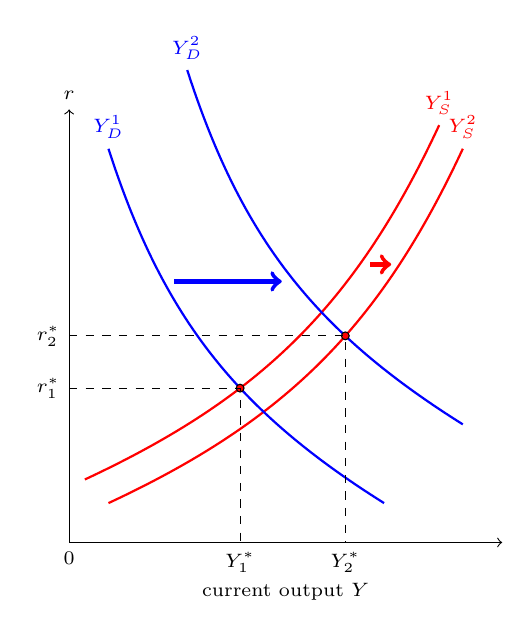
\begin{tikzpicture}[domain=0:5]
                \tikzstyle{every node}=[font=\scriptsize]
                \pgfmathsetmacro{\x}{5};
                \pgfmathsetmacro{\y}{5};
                % \draw[very thin,color=gray, step=0.1] (0,0) grid (\x, \y); % gray grid
                \draw[->] (0,0) node[below]{ $ 0 $  } -- node[below, yshift = -0.4cm]{current output $ Y $} (\x + 0.5,0) ;   % label x axis
                \draw[->] (0,0) -- (0,\y + 0.5) node[above]{$r$} ;   % label y axis
                \draw[thick, red, xshift = -0.3cm, yshift = 0.3cm, name path = aaa]
                    (\x, \y)
                    node[above]{$Y_{S}^{1}$}
                    to[bend left=20]
                    node[pos = 0.3] (AA) {}
                    (0.5, 0.5);
                \draw[thick, red, name path = aa]
                    (\x, \y)
                    node[above]{$Y_{S}^{2}$}
                    to[bend left=20]
                    (0.5, 0.5);
                \draw[thick, blue, name path = bb]
                    (0.5, \y)
                    node[above]{$Y_{D}^{1}$}
                    to[bend right=20]
                    node[pos = 0.3] (BB) {}
                    (4, 0.5);
                \draw[thick, blue, xshift = 1cm, yshift = 1cm, name path = bbb]
                    (0.5, \y)
                    node[above]{$Y_{D}^{2}$}
                    to[bend right=20]
                    (4, 0.5);
                \path[name intersections={of=aaa and bb, by=a}];
                \path[name intersections={of=aa and bbb, by=bbb}];
                \node[draw,fill=red,circle,inner sep=1pt] at (a) {};
                \node[draw,fill=red,circle,inner sep=1pt] at (bbb) {};
                \draw[->, ultra thick, blue] (BB) -- ++(1.5, 0);
                \draw[->, ultra thick, red] (AA) -- ++(0.4, 0);
                \path (a); \pgfgetlastxy{\xcoord}{\ycoord};
                \coordinate (a_x) at (\xcoord, 0);
                \coordinate (a_y) at (0, \ycoord);
                \draw[dashed] (a_y) node[left]{$r_{1}^{*}$}  -- (a) -- (a_x) node[below]{$Y_{1}^{*}$};
                \path (bbb); \pgfgetlastxy{\xcoord}{\ycoord};
                \coordinate (bbb_x) at (\xcoord, 0);
                \coordinate (bbb_y) at (0, \ycoord);
                \draw[dashed] (bbb_y) node[left]{$r_{2}^{*}$}  -- (bbb) -- (bbb_x) node[below]{$Y_{2}^{*}$};

            \end{tikzpicture}
        \end{minipage}
\end{tasks}

% A: z', B: z, C: K, D: G
\Question Using the same figures as in the choice of \ref{z'}, consider a rise in current total factor productivity $ z $. Which of the following figure correctly represents the movement of labor and goods market? \answer{B}

\Question Using the same figures as in the choice of \ref{z'}, consider a rise in government spending $ G $. Which of the following figure correctly represents the movement of labor and goods market? \answer{D}

\Question Using the same figures as in the choice of \ref{z'}, consider a decrease in capital endowment $ K $. Which of the following figure correctly represents the movement of labor and goods market? \answer{C}

\section*{Question 2}
\label{sec:Question_2}
\addcontentsline{toc}{section}{Question 2}

Reference: Lucas human capital accumulation model (1988 JME)

Credit: Julia K. Thomas

Consider a two-period general equilibrium model, where human capital are accumulated by \blue{spending time in education} rather than \blue{purchasing using output goods}.
\begin{itemize}
    \item the utility function is given by $ U(C, C') = u(C) + u(C') $, i.e., consumer doesn't value leisure.
    \item households are endowed with $ H $ of current human capital at date $ 0 $, and they accumulate future human capital $ H' $ by \blue{spending $ 1-\phi $ fraction of their time endowment to education}. The law of motion for human capital is given by
    %
    \begin{equation}
    \label{eq:HlawofMotion}
        H' = H + (1 - \phi )H
    ,\end{equation}
    %
    where $ 1-\phi $ is the fraction of the time endowment that goes to education so that households can accumulate human capital.

    \item households are endowed with $ K $ amount of capital, and determine the investment at date $ 0 $ to determine their future capital $ K' $ at date $ 1 $. The usage of these capital for consumer is to rent to the firm and earn the per-unit rent $ r $.
        The law of motion for physical capital is given by
        %
        \begin{equation}
        \label{eq:KlawofMotion}
            K' = (1-\delta)K + I
        .\end{equation}
    \item Firm's production function is given by
    %
    \begin{equation}
    \label{eq:FirmProduction}
        Y = K^{\alpha} (\phi H)^{1-\alpha};
        Y' = K'^{\alpha} (\phi' H')^{1-\alpha};
    \end{equation}
    %
    Firm pays the per-unit wage $ w $ for the labor supplied by the households and pays per-unit capital renting fee $ r $ to consumers.
    \item Consumer owns the whole firm, and claims the whole profit $ \pi $.
    \item There's no government in this model, i.e., $ G = G' = T = T' = B = 0 $.
\end{itemize}

First, let's construct the budget constraint for consumers.

\Question Consider the current budget constraint, what is the labor income for consumer? \answer{B}
\begin{tasks}(4)
    \task $ r K $
    \task $ w \phi H $
    \task $ w K $
    \task $ r \phi H $
\end{tasks}

\Question Consider the current budget constraint, what is the capital income for consumer? \answer{A}
\begin{tasks}(4)
    \task $ r K $
    \task $ w \phi H $
    \task $ w K $
    \task $ r \phi H $
\end{tasks}

\Question \label{budgetConstrant} What is the current budget constraint for consumer? \answer{D}
\begin{tasks}(2)
    \task $ C \le w H + r \phi K - I + \pi $
    \task $ C \le w \phi H + r \phi K - I + \pi $
    \task $ C \le w H + r K - I + \pi $
    \task $ C \le w \phi H + r K - I + \pi $
\end{tasks}

\Question \label{profit} What is the profit for the firm? \answer{C}
\begin{tasks}(2)
    \task $ \pi = Y - wH - rK $
    \task $ \pi = Y - w\phi H - r \phi K $
    \task $ \pi = Y - w\phi H - rK $
    \task $ \pi = Y - w\phi H - r \phi K $
\end{tasks}

\Question In this economy, does the competitive equilibrium and social planner's problem generate the same result? Why? \answer{B}
\begin{tasks}(1)
    \task No, because the first welfare theorem doesn't holds.
    \task Yes, because the first welfare theorem holds.
    \task Yes, because the first welfare theorem don't holds.
    \task No, because the first welfare theorem holds.
\end{tasks}

Let's solve this model using the social planner's problem.

\Question \label{SPPConsumption} Combine your answers in \ref{budgetConstrant} and \ref{profit}, in the perspective of social planner, we can rewrite household's current budget constraint as \answer{A}
\begin{tasks}(2)
    \task $ C \le Y - I $
    \task $ C \le Y - rK - w\phi H - I $
    \task $ C \le Y - r\phi K - w H - I $
    \task $ C \le Y - r\phi K - w\phi H - I $
\end{tasks}

Since the budget constraint is binding, we can replace consumption as your answer in \ref{SPPConsumption}.

Social planner's problem is then given by

%
%
\begin{align}
        \max_{C, C', \phi, K', H'}
            & u(C) + u(C')
        \\
        \text{ s.t. }
            & C = \text{ your answer in \ref{SPPConsumption} }
        \\
            & C' = Y'
        \\
            & H' = H + (1-\phi)H \label{HLaw}
        \\
            & K' = (1-\delta) K + I \label{KLaw}
\end{align}
%

Replace consumption with your answer in \ref{SPPConsumption} and investment with equation \ref{KLaw}, we can rewrite social planner's problem as
%
\begin{equation*}
    \begin{split}
        \max_{
            \underbrace{
            \text{\answer{C}}
            }_{\text{\ref{argument}}}
        }
            & u(
                \underbrace{
                \text{\answer{A}}
                }_{\text{\ref{Uconsumption}}}
               ) + u(K'^{\alpha} (\phi' H')^{1-\alpha})
        \\
        \text{ s.t. }
            & H' = H + (1-\phi)H
        \\
    \end{split}
\end{equation*}
%

\Question \label{argument}
\begin{tasks}(2)
    \task $\phi, K', H', C'$
    \task $\phi, K', C'$
    \task $\phi, K', H'$
    \task $K', H', C'$
\end{tasks}

\Question \label{Uconsumption}
\begin{tasks}(1)
    \task $ K^{\alpha} (\phi H)^{1-\alpha} + (1-\delta) K - K' $
    \task $ K^{\alpha} (\phi H)^{1-\alpha} $
    \task $ K^{\alpha} (\phi H)^{1-\alpha} + (1-\delta) K - K' + r K $
    \task $ K^{\alpha} (\phi H)^{1-\alpha} + (1-\delta) K - K' + w \phi H $
\end{tasks}

\Question \label{phi'} There's one result directly from our model assumption. Since this is a two-period model, and agents don't live to the third period, we know that $ \phi' =$ \answer{D}
\begin{tasks}(4)
    \task $ 0.3 $
    \task $ 0.5 $
    \task $ 0 $
    \task $ 1 $
\end{tasks}

Using your answer in \ref{phi'} as well as substitute $ H' = (2-\phi)H $ into the utility function, we can write the social planner's problem as
%
\begin{equation*}
    \max_{\phi, K'}
            u(
                \underbrace{
                \text{\answer{A}}
                }_{\text{\ref{Uconsumption}}}
               ) + u(
                \underbrace{
                \text{\answer{C}}
                }_{\text{\ref{UconsumptionPrime}}}
                   )
.\end{equation*}
%

\Question \label{UconsumptionPrime}

\begin{tasks}(2)
    \task $ K'^{\alpha} ( (2-\phi) H)^{-\alpha} $
    \task $ K'^{\alpha} ( (2-\phi) H) $
    \task $ K'^{\alpha} ( (2-\phi) H)^{1-\alpha} $
    \task $ K'^{\alpha} H^{1-\alpha} $
\end{tasks}

\Question \label{FOCK'} The first order condition with respect to $ K' $ would leads to \answer{D}

\begin{tasks}(1)
    \task $ \frac{u'(C)}{u'(C')} = K'^{\alpha} ( (2-\phi) H )^{1-\alpha} $
    \task $ \frac{u'(C)}{u'(C')} = \alpha K'^{\alpha-1} H^{1-\alpha} $
    \task $ \frac{u'(C)}{u'(C')} = K'^{\alpha} ( (2-\phi) H )^{1-\alpha} $
    \task $ \frac{u'(C)}{u'(C')} = \alpha K'^{\alpha-1} ( (2-\phi) H )^{1-\alpha} $
\end{tasks}

\Question \label{FOCphi} The first order condition with respect to $ \phi $ would leads to \answer{B}

\begin{tasks}(1)
    \task $ \frac{u'(C)}{u'(C')} = \left(
        \frac{K'}{K}
    \right)^{1-\alpha} \left(
        \frac{2-\phi}{\phi}
    \right)^{-\alpha}$
    \task $ \frac{u'(C)}{u'(C')} = \left(
        \frac{K'}{K}
    \right)^{\alpha} \left(
        \frac{2-\phi}{\phi}
    \right)^{-\alpha}$
    \task $ \frac{u'(C)}{u'(C')} = \left(
        \frac{K'}{K}
    \right)^{\alpha} $
    \task $ \frac{u'(C)}{u'(C')} = \left(
        \frac{K'}{K}
    \right)^{\alpha-1} \left(
        \frac{2-\phi}{\phi}
    \right)^{-\alpha}$
\end{tasks}

Remember that $ MRS_{C, C'} = \frac{u'(C)}{u'(C')} $, and thus your answer in \ref{FOCK'} and \ref{FOCphi} should equal to each other.

\Question Simplify the above equation and we can get \answer{A}

\begin{tasks}(2)
    \task $ \frac{\phi^{\alpha}}{2-\phi} K'  = \alpha K^{\alpha} H^{1-\alpha}$
    \task $ \frac{\phi^{\alpha}}{2-\phi} K'^{\alpha-1}  = \alpha K^{\alpha} H^{1-\alpha}$
    \task $ \frac{\phi}{2-\phi} K'  = \alpha K^{\alpha} H^{1-\alpha}$
    \task $ \frac{\phi^{1-\alpha}}{2-\phi} K'  = \alpha K^{\alpha} H^{1-\alpha}$
\end{tasks}

From the above equation, we can see that the choice variables, $ \phi $ and $ K' $, are equal to $ \alpha K^{\alpha} H^{1-\alpha} $.
Remember that both $ K $ and $ H $ are the endowments and $ \alpha $ is the parameter of production function.

\Question What is the economics intuition of the this equation? \answer{C}

\begin{tasks}(1)
    \task The investment on human capital is a more favorable option than the investment on physical capital in equilibrium
    \task The investment on human capital is a less favorable option than the investment on physical capital in equilibrium
    \task The investment on human capital and the investment on physical capital are equally favorable options in equilibrium
    \task We cannot determine which investment is more favorable in equilibrium
\end{tasks}








\section*{Question 3}
\label{sec:Question_3}
\addcontentsline{toc}{section}{Question 3}

Credit: Aubhik Khan

Note: In the lecture I only teach two-period model.
This question is meant to be a taste for what graduate level of macroeconomics looks like.
The infinite period model is what most contemporary macroeconomics model looks like, and this question would guide you to solve infinite period model.

Consider the Solow Growth Model.
Labour productivity grows at the rate $\gamma>0$, $X_{t+1}=\left(  1+\gamma\right)  X_{t}$, for $t=0,1,\ldots$, and population grows at the rate $n>0$, $L_{t+1}=\left( 1+n \right)  L_{t}$.
The effective labour force at date $t$ is $N_{t} =X_{t}L_{t}$.
Let aggregate production be given by
\begin{equation}
Y_{t}=AK_{t}^{\alpha}N_{t}^{1-\alpha}\text{ where }0<\alpha<1\text{,}%
\label{production}%
\end{equation}
$A$ is total factor productivity and $K_{t}$ is the present capital stock.
Total consumption is a constant fraction of output,
\begin{equation}
C_{t}=\left(  1-s\right)  Y_{t},\label{consumption}%
\end{equation}
where $0<s<1$ is the savings rate.
There is full depreciation of the capital
stock each period, $\delta=1$. Thus, with $I_{t}$ representing aggregate investment, the capital stock next period is
\begin{equation}
K_{t+1}=I_{t}\text{.}\label{capital}%
\end{equation}
The aggregate resource constraint is
\begin{equation}
C_{t}+I_{t}=Y_{t}.\label{output}%
\end{equation}

\Question \label{IasY} Use \eqref{consumption} to eliminate $C_{t}$ in \eqref{output} and solve for $I_{t}$ in terms of $Y_{t}$ as \answer{D}
\begin{tasks}(4)
    \task $ s C_{t} $
    \task $ (1-s) Y_{t} $
    \task $ (1-s) C_{t} $
    \task $ s Y_{t} $
\end{tasks}

\Question \label{KasY} Substitute your result in \ref{IasY} into \eqref{capital} accumulation process and get $ K_{t+1} $ as \answer{D}
\begin{tasks}(4)
    \task $ s C_{t} $
    \task $ (1-s) Y_{t} $
    \task $ (1-s) C_{t} $
    \task $ s Y_{t} $
\end{tasks}

Define capital per efficiency unit of labour as $k_{t} =\frac{K_{t}}{N_{t}}$ (so that $k_{t+1}=\frac{K_{t+1}}{N_{t+1}}$).

\Question \label{efficiencyLaborUnitGrowthRate} Express $ \frac{N_{t+1}}{N_{t}} $ using only labor productivity growth rate $ \gamma $ and population growth rate $ n $ as \answer{B}
\begin{tasks}(2)
    \task $\gamma n$
    \task $(1+\gamma)(1+n)$
    \task $(1+\gamma)n$
    \task $\gamma(1+n)$
\end{tasks}

\Question \label{Kt+1inYt} Using your answer in \ref{KasY} and express $ \frac{K_{t+1}}{N_{t}} $ using $ Y_{t} $ as \answer{D}
\begin{tasks}(4)
    \task $ \frac{s C_{t}}{N_{t}} $
    \task $ \frac{(1-s) Y_{t}}{N_{t}} $
    \task $ \frac{(1-s) C_{t}}{N_{t}} $
    \task $ \frac{s Y_{t}}{N_{t}} $
\end{tasks}


\Question Find the law of motion of the efficiency unit of capital, i.e., the $ g $ function in $ k_{t+1} = g(k_{t}) $ as \answer{C}
(Hint: $ k_{t+1} = \frac{K_{t+1}}{N_{t+1}} = \frac{N_{t+1}}{N_{t}} \frac{K_{t+1}}{N_{t+1}} $.)
\begin{tasks}(2)
    \task $ k_{t+1} = \frac{sA}{(1+r)n}k_{t}^{\alpha} $
    \task $ k_{t+1} = \frac{s A}{r n} k_{t}^{\alpha} $
    \task $ k_{t+1} = \frac{s A}{(1+r)(1+n)} k_{t}^{\alpha} $
    \task $ k_{t+1} =
    \left(
        \frac{s A}{(1+r)(1+n)} k_{t}
    \right)^{\alpha} $
\end{tasks}


In the infinite period model, what we want to find is ``\blue{steady state}'', which means that ``the variables (called state variables) which define the behavior of the system or the process are unchanging in time.'' (from wikipedia)

\Question Find the steady state efficiency unit of capital of this economy, $ k^{*} $, is \answer{B} (Hint: not changing means $ k_{t+1} = k_{t} = k^{*} $)
\begin{tasks}(2)
    \task $ \left( \frac{sA}{rn }\right)^{\frac{1}{1-\alpha}} $
    \task $ \left( \frac{sA}{(1+r)(1+n) }\right)^{\frac{1}{1-\alpha}} $
    \task $ \left( \frac{sA}{(1+r)n }\right)^{\frac{1}{1-\alpha}} $
    \task $ \left( \frac{sA}{(1+r)(1+n) }\right)^{\frac{\alpha}{1-\alpha}} $
\end{tasks}

\Question \label{kfig} On a figure of $ k_{t} $ on the $ x $-axis and $ k_{t+1} $ on the $ y $-axis, which of the following figure correctly plots the $ g(k_{t}) $ function? \answer{D}

\begin{tasks}(2)
    \task

            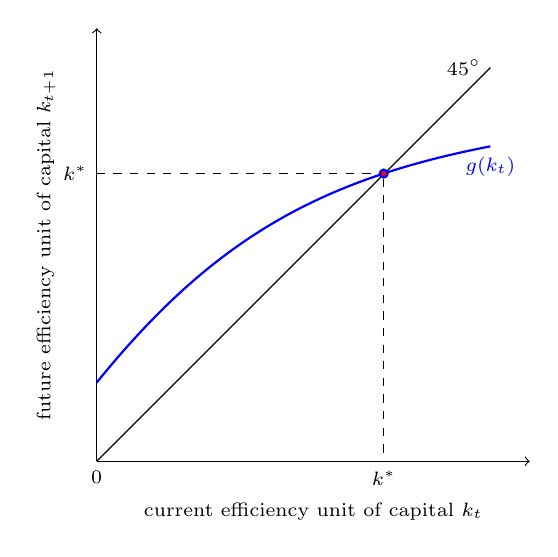
\begin{tikzpicture}[domain=0:5]
                \tikzstyle{every node}=[font=\scriptsize]
                \pgfmathsetmacro{\x}{5};
                \pgfmathsetmacro{\y}{5};
                % \draw[very thin,color=gray, step=0.1] (0,0) grid (\x, \y); % gray grid
                \draw[->] (0,0) node[below]{ $ 0 $  } -- node[below, yshift = -0.4cm]{current efficiency unit of capital $k_{t}$} (\x + 0.5,0) ;   % label x axis
                \draw[->] (0,0) -- node[above, rotate=90, yshift = 0.4cm]{future efficiency unit of capital $k_{t+1}$} (0,\y + 0.5) ;   % label y axis
                \draw[black] plot (\x, \x) node[left]{$45^{\circ}$};
                \draw[thick, blue, yshift = -1cm] (0, 2)
                    to[bend left=20]
                    node[pos=0.21] (b) {}
                    node[pos=0.78,draw,fill=red,circle,inner sep=1pt] (c) {}
                    (5, 5) node[below]{$g(k_{t})$};
                % \draw[shorten >=-1cm, shorten <=-1.5cm, thick, red] (a) -- (b) node[above, yshift=.8cm]{slope $=$ MPC};
                \path (c); \pgfgetlastxy{\xcoord}{\ycoord};
                \coordinate (c_x) at (\xcoord, 0);
                \coordinate (c_y) at (0, \ycoord);
                \draw[dashed] (c_y) node[left]{$k^{*}$}  -- (c) -- (c_x) node[below]{$k^{*}$};
            \end{tikzpicture}
    \task

            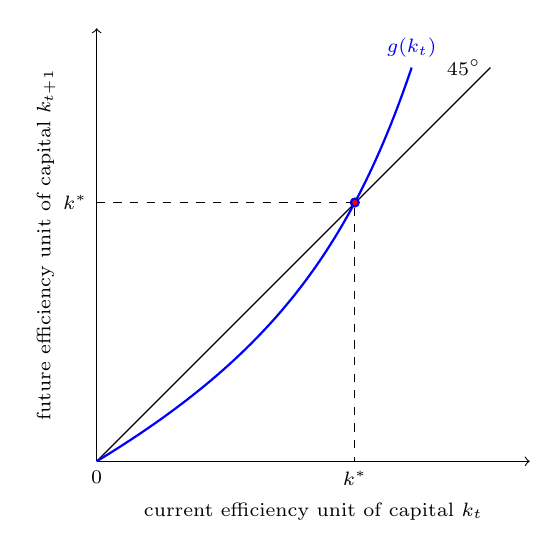
\begin{tikzpicture}[domain=0:5]
                \tikzstyle{every node}=[font=\scriptsize]
                \pgfmathsetmacro{\x}{5};
                \pgfmathsetmacro{\y}{5};
                % \draw[very thin,color=gray, step=0.1] (0,0) grid (\x, \y); % gray grid
                \draw[->] (0,0) node[below]{ $ 0 $  } -- node[below, yshift = -0.4cm]{current efficiency unit of capital $k_{t}$} (\x + 0.5,0) ;   % label x axis
                \draw[->] (0,0) -- node[above, rotate=90, yshift = 0.4cm]{future efficiency unit of capital $k_{t+1}$} (0,\y + 0.5) ;   % label y axis
                \draw[black] plot (\x, \x) node[left]{$45^{\circ}$};
                \draw[thick, blue, yshift = -1cm] (0, 1)
                    to[bend right=20]
                    node[pos=0.21] (b) {}
                    node[pos=0.73,draw,fill=red,circle,inner sep=1pt] (c) {}
                    (4, 6) node[above]{$g(k_{t})$};
                % \draw[shorten >=-1cm, shorten <=-1.5cm, thick, red] (a) -- (b) node[above, yshift=.8cm]{slope $=$ MPC};
                \path (c); \pgfgetlastxy{\xcoord}{\ycoord};
                \coordinate (c_x) at (\xcoord, 0);
                \coordinate (c_y) at (0, \ycoord);
                \draw[dashed] (c_y) node[left]{$k^{*}$}  -- (c) -- (c_x) node[below]{$k^{*}$};
            \end{tikzpicture}
    \task

            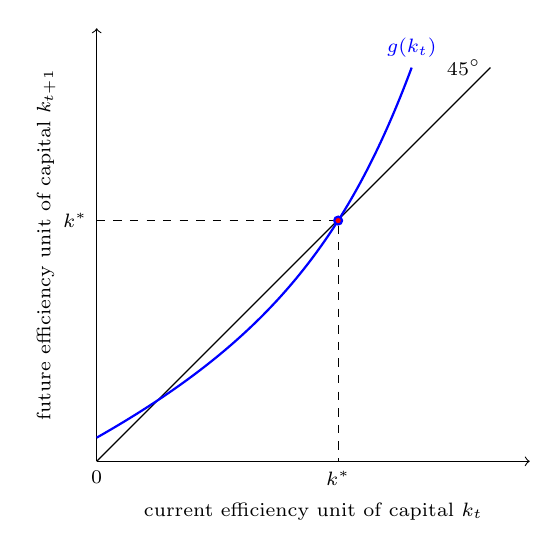
\begin{tikzpicture}[domain=0:5]
                \tikzstyle{every node}=[font=\scriptsize]
                \pgfmathsetmacro{\x}{5};
                \pgfmathsetmacro{\y}{5};
                % \draw[very thin,color=gray, step=0.1] (0,0) grid (\x, \y); % gray grid
                \draw[->] (0,0) node[below]{ $ 0 $  } -- node[below, yshift = -0.4cm]{current efficiency unit of capital $k_{t}$} (\x + 0.5,0) ;   % label x axis
                \draw[->] (0,0) -- node[above, rotate=90, yshift = 0.4cm]{future efficiency unit of capital $k_{t+1}$} (0,\y + 0.5) ;   % label y axis
                \draw[black] plot (\x, \x) node[left]{$45^{\circ}$};
                \draw[thick, blue, yshift = -1cm] (0, 1.3)
                    to[bend right=20]
                    node[pos=0.21] (b) {}
                    node[pos=0.67,draw,fill=red,circle,inner sep=1pt] (c) {}
                    (4, 6) node[above]{$g(k_{t})$};
                % \draw[shorten >=-1cm, shorten <=-1.5cm, thick, red] (a) -- (b) node[above, yshift=.8cm]{slope $=$ MPC};
                \path (c); \pgfgetlastxy{\xcoord}{\ycoord};
                \coordinate (c_x) at (\xcoord, 0);
                \coordinate (c_y) at (0, \ycoord);
                \draw[dashed] (c_y) node[left]{$k^{*}$}  -- (c) -- (c_x) node[below]{$k^{*}$};
            \end{tikzpicture}

    \task

            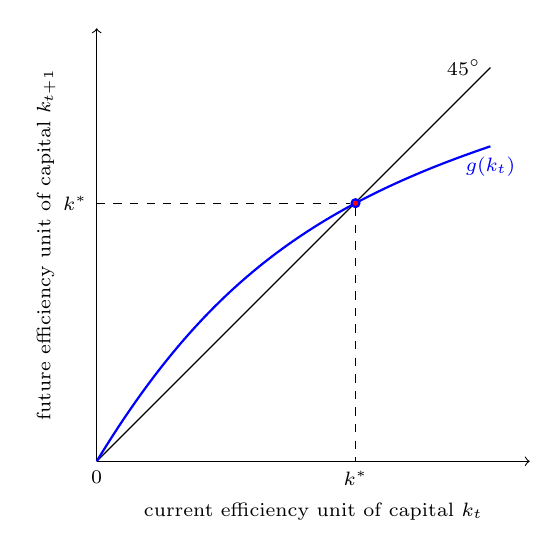
\begin{tikzpicture}[domain=0:5]
                \tikzstyle{every node}=[font=\scriptsize]
                \pgfmathsetmacro{\x}{5};
                \pgfmathsetmacro{\y}{5};
                % \draw[very thin,color=gray, step=0.1] (0,0) grid (\x, \y); % gray grid
                \draw[->] (0,0) node[below]{ $ 0 $  } -- node[below, yshift = -0.4cm]{current efficiency unit of capital $k_{t}$} (\x + 0.5,0) ;   % label x axis
                \draw[->] (0,0) -- node[above, rotate=90, yshift = 0.4cm]{future efficiency unit of capital $k_{t+1}$} (0,\y + 0.5) ;   % label y axis
                \draw[black] plot (\x, \x) node[left]{$45^{\circ}$};
                \draw[thick, blue, yshift = -1cm] (0, 1)
                    to[bend left=20]
                    node[pos=0.21] (b) {}
                    node[pos=0.73,draw,fill=red,circle,inner sep=1pt] (c) {}
                    (5, 5) node[below]{$g(k_{t})$};
                % \draw[shorten >=-1cm, shorten <=-1.5cm, thick, red] (a) -- (b) node[above, yshift=.8cm]{slope $=$ MPC};
                \path (c); \pgfgetlastxy{\xcoord}{\ycoord};
                \coordinate (c_x) at (\xcoord, 0);
                \coordinate (c_y) at (0, \ycoord);
                \draw[dashed] (c_y) node[left]{$k^{*}$}  -- (c) -- (c_x) node[below]{$k^{*}$};
            \end{tikzpicture}
\end{tasks}

\Question What is the $45^{\circ}$ line means in question \ref{kfig}? \answer{B}

\begin{tasks}(3)
    \task $ k_{t+1} > k_{t} $
    \task $ k_{t+1} = k_{t} $
    \task $ k_{t+1} < k_{t} $
\end{tasks}


\Question Among all the figures in the choice of question \ref{kfig}, which graph will the $ g(k_{t}) $ function be \blue{if $ \alpha > 1 $}? \answer{B}

Consider two economies, $a$ and $b$, where economy $b$ has a higher savings rate, \emph{and a higher rate of technological progress}, compared to economy $a$.
In other words, $\gamma_{b}>\gamma_{a}$, and $s_{b}>s_{a}$. Moreover, assume that
\[
\frac{s_{b}}{1+\gamma_{b}}=\frac{s_{a}}{1+\gamma_{a}}\text{,}%
\]
and the rate of population growth is the same ($n_{a}=n_{b}$).

\Question Denote the $ g $ function for both economy as $ g_{a}(k_t) $ and $ g_{b}(k_{t}) $, what is the relationship of two $ g $ function? \answer{B}
\begin{tasks}(1)
    \task $ g_{a}(k_{t}) $ is on top of $ g_{b}(k_t) $, for all $ k_{t} $
    \task $ g_{a}(k_{t}) $ and $ g_{b}(k_t) $ is the same curve
    \task $ g_{a}(k_{t}) $ is below  $ g_{b}(k_t) $, for all $ k_{t} $
    \task $ g_{a}(k_{t}) $ intersects with $g_{b}(k_t) $
\end{tasks}


% Assume both economies have converged to their steady state
% capital by date $T$. If $X_{T}^{a}=X_{T}^{b}$, how
% will income per person differ between economy $a$ and $b$ five years later?
% Explain your answer.




\end{Exercise}




\end{document}
